\documentclass[30pt, french]{tccv}
\usepackage[hmargin=0.2cm,vmargin=0cm]{geometry}
\usepackage{amsfonts} 								% for the \checkmark command 
\usepackage[framemethod=TikZ]{mdframed}						% For box around text
\usepackage[overlay,absolute]{textpos}						% For Textblock
\setlength{\TPHorizModule}{1cm}
\setlength{\TPVertModule}{1cm}
\usepackage{fontspec}								% For extended fonts
\usepackage{enumitem}								% For aptitudes enumeration 








\begin{document}
\begin{upshape}
\fontsize{9pt}{1em}\color{text}\selectfont



%%%%%%%%%%%%%%%%%%%%%%%%%%%%%%%%%%%%%%%%%%%%%%%%%%%%%%%%%%%%%%%%%%%%%%%%%%%%%%%%%%%%%%%%%%%%%%%%%%%%%%%%%%%%%%%%%%%%%%%%%%%%%%%%%%%%%%%%%%%%%%%%%%%%%%%%%%%%%%%%%%%%%%
%
%			0/ HEADER
%
%%%%%%%%%%%%%%%%%%%%%%%%%%%%%%%%%%%%%%%%%%%%%%%%%%%%%%%%%%%%%%%%%%%%%%%%%%%%%%%%%%%%%%%%%%%%%%%%%%%%%%%%%%%%%%%%%%%%%%%%%%%%%%%%%%%%%%%%%%%%%%%%%%%%%%%%%%%%%%%%%%%%%%




\begin{textblock}{6.5}(0.5,0.5)
\personal
    []
    {923 Route de la Roque sur Pernes 
    84800 Isle sur la Sorgue}
    {+33 6 79 59 85 38}
    {anne.martinez.sandoval@gmail.com}
\end{textblock}

\begin{textblock}{21}(0,1)
     \centering{\headerfirstnamestyle{Anne}   \headerlastnamestyle{Martinez}}
\end{textblock}

\begin{textblock}{21}(17.5,0.5)
		%%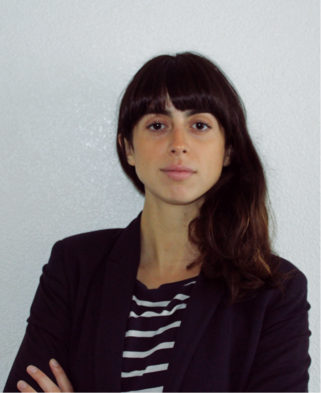
\includegraphics[width=3cm]{../Figure/Rocio3.png}
\end{textblock}  



\begin{textblock}{21}(0,2.3)

\begin{center}
\fontsize{10pt}{1.5em}\color{text}\bodyfontlight\upshape\selectfont

	{\fontsize{14pt}{5em}\scshape\bfseries \'Etudiante en communication\\} 

	\vspace{5pt}
Œuvrer dans un environnement de travail au sein d’une institution internationale représentant de nouveaux et constants défis afin de développer mes capacités et acquérir de nouvelles connaissances. 
\end{center}
\end{textblock}  





%%%%%%%%%%%%%%%%%%%%%%%%%%%%%%%%%%%%%%%%%%%%%%%%%%%%%%%%%%%%%%%%%%%%%%%%%%%%%%%%%%%%%%%%%%%%%%%%%%%%%%%%%%%%%%%%%%%%%%%%%%%%%%%%%%%%%%%%%%%%%%%%%%%%%%%%%%%%%%%%%%%%%%
%
%			1/ EDUCATION
%
%%%%%%%%%%%%%%%%%%%%%%%%%%%%%%%%%%%%%%%%%%%%%%%%%%%%%%%%%%%%%%%%%%%%%%%%%%%%%%%%%%%%%%%%%%%%%%%%%%%%%%%%%%%%%%%%%%%%%%%%%%%%%%%%%%%%%%%%%%%%%%%%%%%%%%%%%%%%%%%%%%%%%%

\begin{education}
\vspace{0.5cm}
\item[Master 1 Science politique et Relations Internationales]{2016 -- 2017}
     {Lobatchevski Université, Russie}
     {Année d’échange}


\vspace{0.5cm}
\item[Licence en Science Politique et Relations Internationales]{2014 -- 2015}
     {Centro de Investigación y Docencia Económicas (CIDE), Méxique}
     {Année d’échange}

     
\vspace{0.5cm}    
\item[Licence en Science Politique ]{2012 -- 2014}
     {Université Lumière Lyon 2, France}
     {Mention bien}

     
\vspace{0.5cm}
\item[Baccalauréat Économique et Social]{2008 -- 2010}
     {}
     {Mention bien}


\end{education}


%%%%%%%%%%%%%%%%%%%%%%%%%%%%%%%%%%%%%%%%%%%%%%%%%%%%%%%%%%%%%%%%%%%%%%%%%%%%%%%%%%%%%%%%%%%%%%%%%%%%%%%%%%%%%%%%%%%%%%%%%%%%%%%%%%%%%%%%%%%%%%%%%%%%%%%%%%%%%%%%%%%%%%
%
%			2/ COMPETENCE
%
%%%%%%%%%%%%%%%%%%%%%%%%%%%%%%%%%%%%%%%%%%%%%%%%%%%%%%%%%%%%%%%%%%%%%%%%%%%%%%%%%%%%%%%%%%%%%%%%%%%%%%%%%%%%%%%%%%%%%%%%%%%%%%%%%%%%%%%%%%%%%%%%%%%%%%%%%%%%%%%%%%%%%%


\begin{competence}


\section{Compétences linguistiques}
\begin{factlist}
\item{Français} {Langue maternelle}	
\item{Espagnol} {Bilingue}	
\item{Anglais} {Confirmé}	
\item{Russe} {Avancé}
\end{factlist}


\vspace{0.5cm}
\section{Aptitudes}
\begin{itemize}[leftmargin=13pt]
  \setlength\itemsep{-3pt} 
  \cvitem[\checkmark]  Connaissances de la situation des Droits de l’Homme au Mexique
  \cvitem[\checkmark]  Analyse de discours officiels et comparaison avec les statistiques
  \cvitem[\checkmark]  Connaissances des politiques migratoires entre le Canada-Etats-Unis-Mexique
  \cvitem[\checkmark]  Rédaction et traduction de discours officiels
  \cvitem[\checkmark]  Organisation d’événements officiels
  \cvitem[\checkmark]  Traduction français-espagnol et anglais-espagnol
  \cvitem[\checkmark]  Maîtrise des réseau sociaux ainsi que des OS Windows et Mac. 
\end{itemize}



\end{competence}




%%%%%%%%%%%%%%%%%%%%%%%%%%%%%%%%%%%%%%%%%%%%%%%%%%%%%%%%%%%%%%%%%%%%%%%%%%%%%%%%%%%%%%%%%%%%%%%%%%%%%%%%%%%%%%%%%%%%%%%%%%%%%%%%%%%%%%%%%%%%%%%%%%%%%%%%%%%%%%%%%%%%%%
%
%			3/ EXPERIENCE
%
%%%%%%%%%%%%%%%%%%%%%%%%%%%%%%%%%%%%%%%%%%%%%%%%%%%%%%%%%%%%%%%%%%%%%%%%%%%%%%%%%%%%%%%%%%%%%%%%%%%%%%%%%%%%%%%%%%%%%%%%%%%%%%%%%%%%%%%%%%%%%%%%%%%%%%%%%%%%%%%%%%%%%%


\begin{experience}

\vspace{2cm}
\item{\color{text} Octobre 2015 -- Main 2016}
     {Université de Rennes 1}
     {Tutrice}
     \fontsize{9pt}{1em}\color{text}\bodyfontlight\upshape\selectfont
     
     Tutrice au Bureau des Affaires Internationales de la faculté Droit/Science Politique

 
\vspace{3cm}
\item{Septembre 2014 -- Mars 2015}
     {Ambassade de Belgique à Mexico, Mexique}
     {Attachée de presse}
     \fontsize{9pt}{1em}\color{text}\bodyfontlight\upshape\selectfont

     Analyse et suivi de l’information des contenus digitaux générée par les médias (officiels et non officiels) afin de faciliter l’identification de thèmes politiques et sociaux. \\
     Rédaction de synthèses sur l’actualité politique et sociale mexicaine destinées au siège à Bruxelles.

\end{experience}






\end{upshape}
\end{document}
